\subsubsection{Hardware Design Understanding: Timeline Interface Analysis}

The timeline interface analysis is described in Section~\ref{sec:client-timeline};
this section focuses on its evaluation (Figure~\ref{fig:eval-timeline}).

\begin{figure}[tp]
    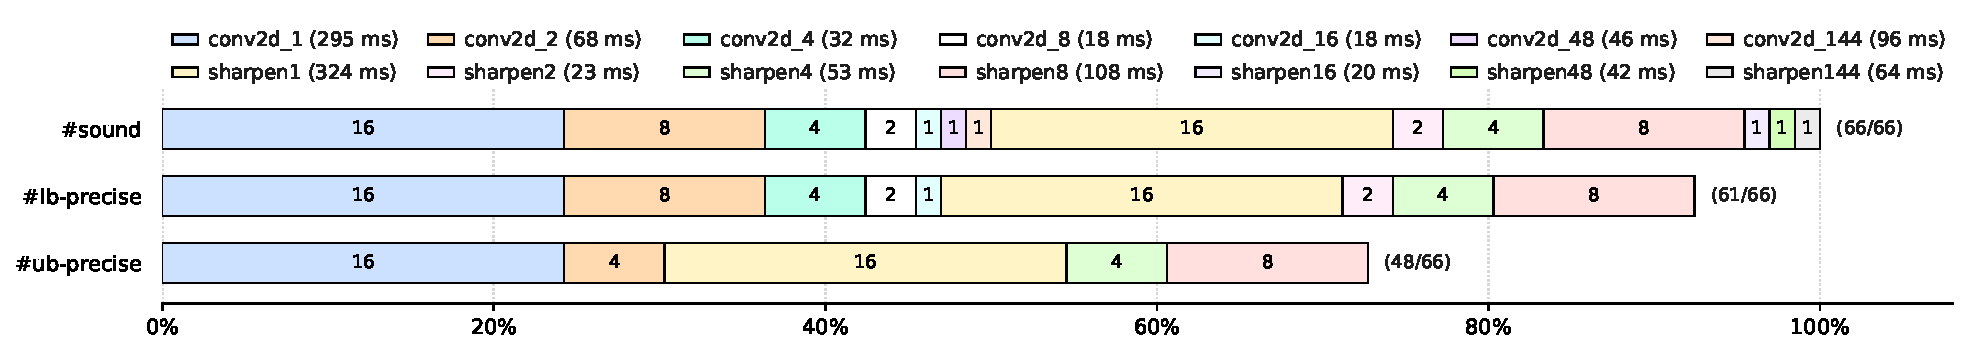
\includegraphics[width=\linewidth,clip,trim=8 9 11 15]{figures/timeline-eval}
    \caption{
        Evaluation of timeline interface analysis (a hardware design understanding client built on top of \tia), where \texttt{\#sound} denotes the number of inferred timeline intervals that are supersets of the corresponding ground-truth intervals (recall: 100\%),
        \texttt{\#lb-precise} denotes the number of inferred timeline intervals with a precise lower bound (lower-bound precision: 92.4\%), and
        \texttt{\#up-precise} denotes the number of inferred intervals with a precise upper bound (upper-bound precision: 72.7\%).
        Analysis times are shown in parentheses.
    }\label{fig:eval-timeline}
\end{figure}

\paragraph{Benchmarks}

Our timeline interface analysis is inspired by the hardware timeline type system~\cite{nigam_modular_2023}, which specifies the clock-cycle intervals during which each input or output is required or available, providing a convenient interface for hardware designers to understand the temporal behavior of a hardware module.
We therefore reuse the hardware designs evaluated in~\cite{nigam_modular_2023}, whose timeline interfaces are established by the type system, as benchmarks for evaluating our timeline interface analysis.
The benchmarks include 14 designs, shown in Figure~\ref{fig:eval-timeline}, implementing two image-processing accelerator kernels (\texttt{conv2d} and \texttt{sharpen}), with 7 design points for each kernel representing different resource-throughput trade-offs.

\paragraph{Understanding the Results}

Figure~\ref{fig:eval-timeline} presents the results of timeline interface analysis.
Across the 66 top-module output ports in the benchmarks, our timeline interface analysis infers 66 timeline intervals with the following results.
\emph{First}, all 66 inferred intervals are sound, i.e., they are supersets of the corresponding ground-truth intervals, yielding a recall of 100\%.
\emph{Second}, 61 inferred intervals have a precise lower bound, yielding a lower-bound precision of $61/66 = 92.4\%$.
\emph{Third}, 48 inferred intervals have a precise upper bound, yielding an upper-bound precision of $48/66 = 72.7\%$.
Thus, the upper-bound precision is lower than the lower-bound precision.

The lower upper-bound precision is primarily caused by imprecision in the underlying \tia, which can introduce false-positive temporal influences at larger, potentially unbounded clock cycles due to widening and path insensitivity.
For example, in \texttt{conv2d\_4}, each output has a ground-truth timeline interval of $[G+6, G+7)$, whereas our timeline interface analysis reports $[G+6, G+9)$.
Although the inferred interval is sound and has a precise lower bound, its upper bound is imprecise because the underlying \tia reports two false-positive temporal influence objects at clock cycles 7 and 8.
In the worst case, the inferred upper bound is infinity, which occurs for 4 of the 66 ports.
For example, the output port $O$ of \texttt{conv2d\_48} has a ground-truth timeline interval of $[G+12, G+13)$, whereas our analysis reports $[G+9, G+\infty)$.
This imprecision arises because path insensitivity in the underlying \tia can introduce a loop in the temporal influence graph (TIG), causing infinitely many temporal influences to propagate to $O$ and resulting in an infinite upper bound, as described in Section~\ref{sec:client-timeline}.
We think improving the precision of \tia in future work could improve the precision of this hardware design understanding client.

As indicated by the analysis times in parentheses to the right of the benchmark names in Figure~\ref{fig:eval-timeline}, our timeline interface analysis is efficient, taking an average analysis time of 86.2 milliseconds across the benchmarks, including the time spent by the underlying \tia.
This efficiency stems from both the efficiency of \tia and the lightweight reuse of its computed temporal influence information: the client analysis only queries \tia's results to compute the minimal interval containing all clock cycles occurring in the temporal influence objects, as described in Section~\ref{sec:client-timeline}, and therefore incurs little additional computational overhead.
